% ============================================================
% 07_resultados.tex
% ============================================================

\section{Resultados y Validación}
\label{sec:resultados}

\subsection{Comportamiento del firmware}

La validación del firmware se realizó mediante pruebas funcionales sobre el
prototipo físico, monitorizando la salida del puerto serie (JTAG/USB) mediante
el monitor del ESP-IDF (\texttt{idf.py monitor}). Las pruebas abarcaron los
siguientes escenarios:

\subsubsection{Inicialización del sistema}

Al arrancar, el sistema produce la secuencia de log esperada indicando el estado de
cada periférico:

\begin{lstlisting}[caption={Log de inicialización del firmware (extracto representativo).}, label={lst:log_init}]
I (502) control-luz: === Control Luz (logica + MQTT) ===
I (1234) control-luz: BH1750 ventana: OK, aula: OK, SHT30: OK
I (1234) control-luz: listo: bajo 60 lx / alto 100 lx, reposo tras 300 s
I (2100) control-luz: WiFi conectado
I (2340) control-luz: MQTT conectado
\end{lstlisting}

\subsubsection{Control de iluminación}

Se verificó el comportamiento de la lógica de control bajo los escenarios descritos
en la Tabla~\ref{tab:pruebas_logica}. En todos los casos, el relé respondió
conforme a lo esperado por la función \texttt{regla\_deseado()}, con el debounce
de 2\,s correctamente aplicado.

\begin{table}[htbp]
  \caption{\textit{Escenarios de prueba de la lógica de control de iluminación.}}
  \label{tab:pruebas_logica}
  \centering
  \small
  \begin{tabularx}{\textwidth}{@{}p{3.5cm}p{2.5cm}p{2.5cm}Xp{2cm}@{}}
    \toprule
    \textbf{Escenario} & \textbf{Lux ventana} & \textbf{Lux aula} & \textbf{Presencia} & \textbf{Relé esperado} \\
    \midrule
    Día soleado, aula vacía     & $>$100\,lx & —      & No & OFF \\
    Día soleado, aula ocupada   & $>$100\,lx & —      & Sí & OFF \\
    Nublado, aula ocupada       & 40\,lx    & 70\,lx & Sí & ON  \\
    Nublado, foco encendido     & 40\,lx    & 150\,lx & Sí & ON (mantiene) \\
    Umbral de histéresis        & 70–100\,lx & —     & Sí & mantiene \\
    Sin presencia (5\,min)      & 40\,lx    & 90\,lx & No & OFF \\
    Sensor ventana en falla     & falla     & 55\,lx & Sí & ON  \\
    Ambos sensores en falla     & falla     & falla  & Sí & mantiene \\
    \bottomrule
  \end{tabularx}
  \vspace{4pt}

  \noindent\textit{Nota.} Los umbrales configurados son: umbral bajo = 60\,lx,
  umbral alto = 100\,lx. El estado ``mantiene'' indica que el relé conserva
  su estado previo sin cambios.
\end{table}

\subsubsection{Sensor de presencia}

El radar LD2420 fue evaluado en un ambiente de laboratorio. Se verificó la
detección de movimiento en el rango configurado (20–400\,cm) y la no activación
ante objetos estáticos sin presencia humana. El diagnóstico de inicio del radar
(\texttt{diagnosticar\_radar()}) reportó correctamente la recepción de tramas
válidas dentro de los primeros 20\,s de operación. La lógica de votación de 2
evidencias en 500\,ms demostró ser efectiva para eliminar falsos positivos
ocasionales del sensor.

\subsubsection{Publicación MQTT y latencia}

Se midió el tiempo transcurrido entre el cambio de estado del relé y la publicación
de la telemetría correspondiente. Dado que la bandera \texttt{publicar\_ya} se
activa en el mismo ciclo de 20\,ms que detecta el cambio y la publicación se
realiza en la siguiente iteración condicionada a la disponibilidad de la conexión
MQTT, la latencia de publicación ante evento oscila entre 20\,ms y 60\,ms bajo
condiciones normales de red.

La publicación periódica de 60\,s fue verificada mediante el monitor de
Node-RED, observándose inserciones regulares en la base de datos SQLite.

\subsection{Integración del stack servidor}

\subsubsection{Inicialización de la base de datos}

El flujo \textit{Init DB} de Node-RED se ejecutó correctamente al iniciar el
contenedor, creando las tres tablas (\texttt{nodes}, \texttt{telemetry},
\texttt{node\_config}) y ejecutando las migraciones de esquema. Se verificó que
las migraciones son idempotentes: una segunda ejecución no produce errores ni
modifica datos existentes.

\subsubsection{Detector de nodos fuera de línea}

El flujo \textit{Offline Detector} fue validado desconectando físicamente el nodo
ESP32-C3 durante más de 60\,s. Transcurrido ese tiempo, el nodo fue marcado como
\texttt{is\_online = 0} en la base de datos, y la interfaz web reflejó el cambio
de estado (badge \textit{Offline}) en la siguiente consulta periódica de 15\,s.

\subsubsection{API REST}

Los diez endpoints de la API fueron probados mediante solicitudes HTTP directas
desde la interfaz web y con herramientas de línea de comandos. Se verificó la
correcta respuesta JSON de cada endpoint, el manejo del código 400 cuando faltan
parámetros requeridos y el código 405 en el intento de modificar umbrales del
firmware.

\subsection{Interfaz web}

La Figura~\ref{fig:prototipo} reserva el espacio para fotografías del prototipo físico.

\begin{figure}[htbp]
  \centering
  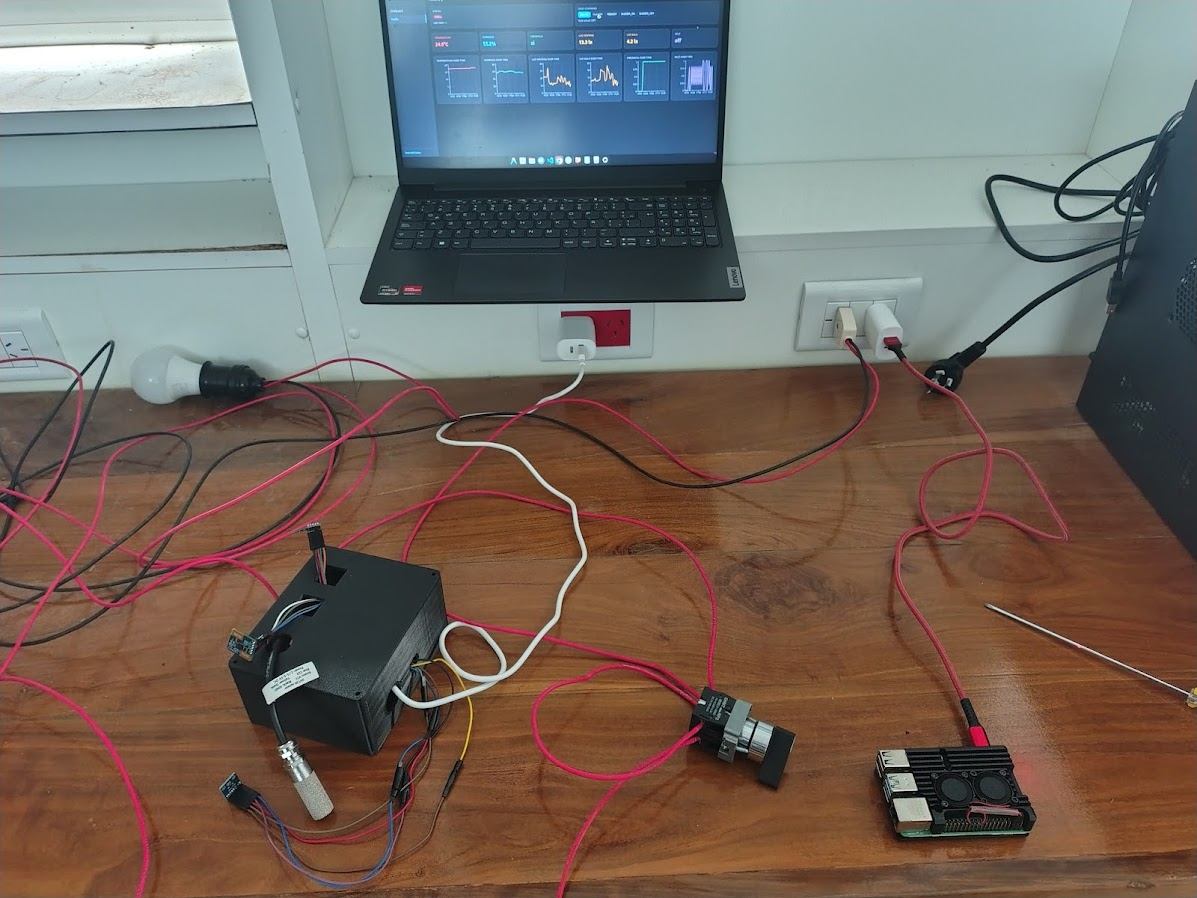
\includegraphics[width=0.95\textwidth]{figuras/proto.jpg}

  \caption{\textit{Prototipo funcional del nodo sensor NodeAlert IoT: ESP32-C3 SuperMini con sensores BH1750, SHT30 y LD2420.}}
  \label{fig:prototipo}
\end{figure}

La interfaz web se validó en un navegador de escritorio. Se comprobó la
actualización automática del Dashboard cada 10\,s, la navegación entre vistas,
el envío del comando REBOOT desde la vista de detalle (que produjo el reinicio
del nodo en aproximadamente 2\,s), y la visualización de los gráficos de serie
temporal con las últimas 50 lecturas.

\subsection{Resumen de requisitos cumplidos}

La Tabla~\ref{tab:requisitos} presenta la relación entre los requisitos mínimos
de la cátedra y el elemento del sistema que los satisface.

\begin{table}[htbp]
  \caption{\textit{Verificación de los requisitos mínimos de la cátedra.}}
  \label{tab:requisitos}
  \centering
  \small
  \begin{tabularx}{\textwidth}{@{}p{5.5cm}X@{}}
    \toprule
    \textbf{Requisito} & \textbf{Elemento que lo satisface} \\
    \midrule
    Programación de microcontrolador & ESP32-C3 con firmware ESP-IDF en C \\
    Lógica de muestreo y optimización & Bucle 20\,ms, lectura cada 1\,s, publicación cada 60\,s \\
    Modos de ahorro de energía & No implementado (monitoreo en tiempo real) \\
    Comunicación bidireccional micro--computador & MQTT: telemetría (ESP32$\rightarrow$RPi) y comandos (RPi$\rightarrow$ESP32) \\
    Protocolo MQTT para IoT & Cliente MQTT ESP-IDF sobre red Wi-Fi 802.11 \\
    Configuración propia de broker & Mosquitto con ACL y autenticación en Docker \\
    Suscriptores y publicadores & ESP32 publica telemetría; Node-RED suscribe; Node-RED publica comandos; ESP32 suscribe \\
    Interfaz de usuario & Frontend React con Dashboard, Nodes y NodeDetail \\
    Visualización de variables medidas & Tarjetas de valores actuales y gráficos temporales en React \\
    Controles de interacción & Botones REBOOT, BUZZER\_ON/OFF, creación/eliminación de nodos \\
    \bottomrule
  \end{tabularx}
  \vspace{4pt}

  \noindent\textit{Nota.} RPi = Raspberry Pi. Los comandos BUZZER\_ON/OFF son
  recibidos por el nodo, que en la implementación actual los mapea al control del LED
  de presencia, dado que el hardware no incluye buzzer físico.
\end{table}

